% =============================================================================
%  Final (Phase II) IEEE report - Systolic Array Matrix Multiplication Accelerator
%  Course : CSA-222 Modern Computer Architecture
%  Build  : pdflatex final_report.tex  (run twice)   -- or upload to Overleaf
%  Figures: ../docs/figures/*.png and ../results/figures/*.png
% =============================================================================
\documentclass[conference]{IEEEtran}
\IEEEoverridecommandlockouts
\usepackage{cite}
\usepackage{amsmath,amssymb}
\usepackage{graphicx}
\usepackage{booktabs}
\usepackage{array}
\usepackage{multirow}
\usepackage{xcolor}
\usepackage{url}
\usepackage[hidelinks]{hyperref}
\graphicspath{{../docs/figures/}{../results/figures/}}

\begin{document}

\title{Design and Evaluation of a 4$\times$4 Output-Stationary Systolic Array Accelerator for Fixed-Point Matrix Multiplication}

\author{
\IEEEauthorblockN{Harshvardhan Gupta}
\IEEEauthorblockA{2401010185}
\and
\IEEEauthorblockN{Harsha Gonela}
\IEEEauthorblockA{2401010181}
\and
\IEEEauthorblockN{Abhijeet Dey}
\IEEEauthorblockA{2401010014}
\and
\IEEEauthorblockN{Saumya Kumar}
\IEEEauthorblockA{2401010432}
\and
\IEEEauthorblockN{Shivansh Upadhyay}
\IEEEauthorblockA{2401020109}
\and
\IEEEauthorblockA{\parbox{0.9\textwidth}{\centering
\textit{B.Tech CS\&AI / CS\&DS, Semester 5 --- CSA-222 Modern Computer Architecture}\\
\textit{Newton School of Technology}\\
GitHub: \url{https://github.com/Harsh-gupta-07/MCA-Phase1}}}
}

\maketitle

% -----------------------------------------------------------------------------
% abstract_intro.tex  -- written by Harshvardhan
\begin{abstract}
Matrix multiplication dominates the arithmetic of modern machine-learning
workloads, and general-purpose processors execute it inefficiently because
every multiply-accumulate (MAC) operation re-fetches its operands. Systolic
arrays, the structure at the core of Google's Tensor Processing Unit, reuse
each operand across a row or column of processing elements (PEs). This paper
presents the complete design and evaluation of a synthesizable, parameterised
$N\times N$ output-stationary systolic-array accelerator in Verilog-2005,
built around signed Q4.4 operands and 32-bit accumulators. Phase~I delivered
a verified $4\times4$ prototype. Phase~II adds row-wide double-buffered
(ping-pong) operand buffers, a result buffer, back-to-back and accumulate
modes, output requantisation with saturation, hardware performance
counters, optional pipeline registers, a sequential single-MAC baseline
and a weight-stationary comparison array. More than 85\,000 element-level
checks, including a 1000-matrix random regression, pass against a bit-exact
Python golden model. A row-wide interface and overlapping data transfer
with computation bring the cost of a $4\times4$ product from 60 to 12
cycles. Two pipeline registers
raise the post-route clock on a Lattice ECP5 FPGA from 51 to 116~MHz, so a
$4\times4$ product completes every 121~ns: 12.4$\times$ faster than the
sequential baseline, using 16 DSP blocks. A cycle-exact analytical model
predicts every measured latency, and the comparison with a
weight-stationary array explains why output-stationary utilisation is
capped at one third.
\end{abstract}

\begin{IEEEkeywords}
systolic array, matrix multiplication, processing element, MAC,
fixed-point arithmetic, double buffering, FPGA, Verilog
\end{IEEEkeywords}

% -----------------------------------------------------------------------------
\section{Introduction}
As Dennard scaling ended, performance growth moved from faster general-purpose
cores to \emph{domain-specific architectures}~\cite{hennessy2019golden}. Deep
learning is the most prominent target. Its fully connected and convolutional
layers reduce to general matrix multiplication (GEMM)~\cite{sze2017efficient}.
On a CPU, a GEMM triple loop is limited by the memory wall: each MAC needs two
operand loads. A \emph{systolic array}~\cite{kung1979systolic,kung1982why}
instead passes operands between neighbouring PEs, so an operand fetched once
feeds a whole row or column. The result is high throughput, short wires and
a regular structure.

This project designs, verifies and evaluates a small systolic GEMM
accelerator, in line with Module~6 of the course (heterogeneous computing,
TPU/AI hardware). It builds on the digital-design foundations of
Modules~1--2 and on the performance concepts of Modules~4--5 (CPI, Amdahl's
law, pipelining)~\cite{patterson_cod,harris_ddca}. The work is entirely
simulation and synthesis based; no board is required. The contributions are:
\begin{itemize}
\item a parameterised output-stationary (OS) array with a complete host
interface, double buffering, accumulate mode and on-chip performance counters;
\item a sequential single-MAC baseline and a weight-stationary (WS) streaming
array, both verified, for quantitative comparison;
\item a verification environment of 10 self-checking testbenches driven by a
bit-exact golden model;
\item post-route timing and resource results, a pipelining study and a
cycle-exact analytical performance model.
\end{itemize}

% literature.tex  -- written by Harsha
\section{Literature Review}

\subsection{Systolic Computing}
Kung and Leiserson introduced systolic arrays for VLSI matrix
computations~\cite{kung1979systolic}. Kung later characterised them by
rhythmic data flow, high operand reuse, nearest-neighbour communication
and simple replicated cells~\cite{kung1982why}. These are the same
data-parallel principles that underlie SIMD and multiprocessor
design~\cite{culler_pca}.

\subsection{Systolic Arrays in AI Accelerators}
Google's TPU~\cite{jouppi2017tpu} uses a $256\times256$ weight-stationary
array of 8-bit MACs (92~TOPS). It is fed from a unified buffer and a
double-buffered weight FIFO, so that data movement overlaps computation.
Later generations keep the systolic core~\cite{jouppi2021tpuv4i}.
Gemmini~\cite{genc2021gemmini} generates parameterised systolic
accelerators for RISC-V SoCs and supports both OS and WS dataflows.
SCALE-Sim~\cite{samajdar2018scalesim} models array size, dataflow and buffer
effects. All three works show that \emph{data movement and buffering},
not the MAC itself, often decide real throughput. Phase~II of this project
confirms this observation quantitatively.

\subsection{Dataflow Taxonomy}
Sze \emph{et al.}~\cite{sze2017efficient} classify accelerators by which
operand stays in the PE (Table~\ref{tab:dataflow}). Weight-stationary
designs (TPU) preload $B$ and move partial sums. Output-stationary designs
(ShiDianNao~\cite{du2015shidiannao}) keep $C_{ij}$ in place and stream $A$
and $B$. Row-stationary designs (Eyeriss~\cite{chen2017eyeriss}) maximise
reuse in convolutions. We implement OS as the main design and WS as a
measured alternative.

\begin{table}[t]
\centering
\caption{Systolic dataflows}
\label{tab:dataflow}
\setlength{\tabcolsep}{3pt}
\begin{tabular}{@{}lccc@{}}
\toprule
 & \textbf{Weight-st.} & \textbf{Output-st.} & \textbf{Row-st.}\\
\midrule
Resident in PE & $B$ (weights) & $C$ (psum) & filter row \\
Moving operands & $A$, psum & $A$, $B$ & mixed \\
Vertical link width & 32 b (psum) & 8 b ($B$) & mixed \\
Example & TPU~\cite{jouppi2017tpu} & ShiDianNao~\cite{du2015shidiannao} & Eyeriss~\cite{chen2017eyeriss}\\
\bottomrule
\end{tabular}
\end{table}

\subsection{Fixed-Point Arithmetic}
Jacob \emph{et al.}~\cite{jacob2018quantization} showed that 8-bit integer
inference loses little accuracy compared with floating point, while an
8-bit multiplier is far cheaper. Production accelerators therefore pair
8-bit operands with 32-bit accumulators and requantise the
outputs~\cite{jouppi2017tpu}. We follow this scheme with Q4.4 operands, a
Q24.8 accumulator and Q4.4 requantised outputs.

\subsection{Positioning}
Industrial arrays are too large to study in a course project. Our design
is small enough to simulate exhaustively with open-source tools, yet it
exposes the same trade-offs: latency versus throughput, PE count versus
cycles, buffering versus area, clock frequency versus pipeline depth, and
dataflow choice.

% solution.tex  -- written by Saumya
\section{Proposed Solution}

\subsection{System Architecture}
Fig.~\ref{fig:system} shows the final accelerator
(\texttt{systolic\_top\_v2}); the blocks added in Phase~II are outlined.
The host writes one row of $A$ or $B$ per cycle into the \emph{shadow} bank
of the ping-pong buffers. A \texttt{start} pulse swaps the banks, and the
controller streams column $k$ of $A$ and row $k$ of $B$ into the skew
buffers. The skew buffers stagger them into the diagonal wavefront needed
by the $4\times4$ PE array. On completion the accumulators are copied into a
result buffer, from which the host reads one row of $C$ per cycle, either
raw (Q24.8) or requantised (Q4.4). Table~\ref{tab:modules} lists the RTL
hierarchy. The Phase~I top level (\texttt{systolic\_top}) is kept unchanged
as a comparison point.

\begin{figure*}[t]
\centering
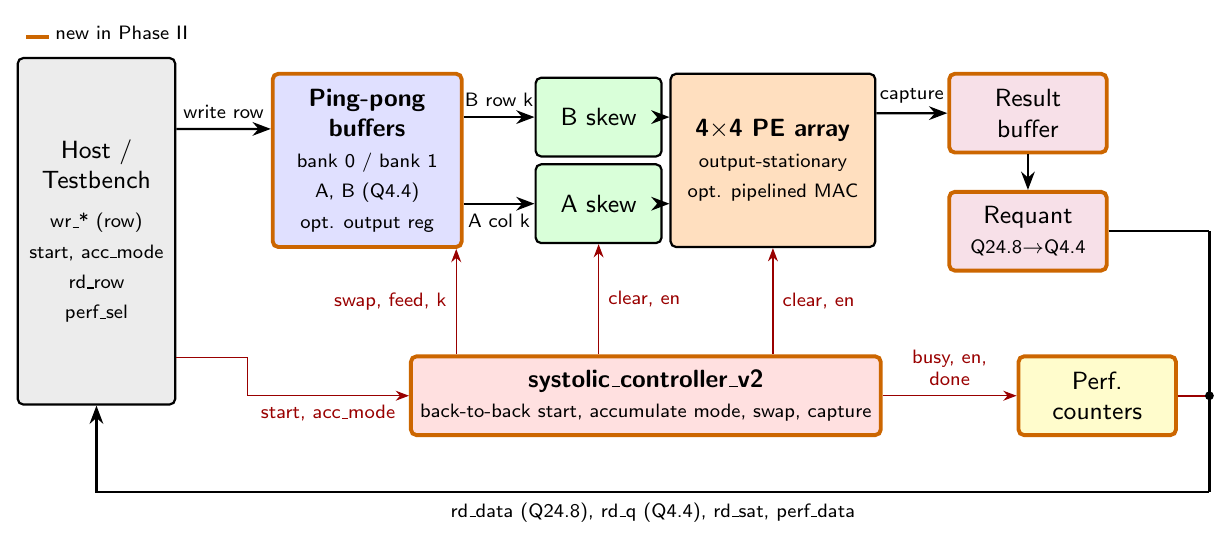
\includegraphics[width=0.86\textwidth]{fig_system_v2.png}
\caption{Final accelerator \texttt{systolic\_top\_v2}. Orange outlines mark blocks added in Phase~II.}
\label{fig:system}
\end{figure*}

\begin{table}[t]
\centering
\caption{RTL modules (Verilog-2005)}
\label{tab:modules}
\setlength{\tabcolsep}{2.5pt}
\begin{tabular}{@{}lp{4.75cm}@{}}
\toprule
\textbf{Module} & \textbf{Function} \\
\midrule
\texttt{mac\_unit} & Q4.4$\times$Q4.4 MAC, 32-bit acc., opt.\ pipeline \\
\texttt{pe} & MAC + east/south forwarding registers \\
\texttt{systolic\_array} & $N\times N$ PE grid (\texttt{generate}) \\
\texttt{input\_skew} & lane $k$ delayed by $k$ cycles \\
\texttt{matrix\_buffer\_pp} & ping-pong $A$/$B$ banks, row writes \\
\texttt{systolic\_controller\_v2} & FSM: back-to-back, accumulate, swap \\
\texttt{requant} & Q24.8$\to$Q4.4, round + saturate \\
\texttt{perf\_counters} & cycle / busy / product counters \\
\texttt{systolic\_top\_v2} & integration + result buffer \\
\midrule
\texttt{seq\_matmul} & baseline: one MAC, $N^3$ cycles \\
\texttt{pe\_ws}, \texttt{ws\_top} & weight-stationary streaming array \\
\texttt{systolic\_top} & Phase~I top (element-wise interface) \\
\bottomrule
\end{tabular}
\end{table}

\subsection{Number Representation and Requantisation}
Operands are signed Q4.4 (range $[-8, 7.9375]$, resolution $0.0625$).
Their product is exact in Q8.8 and is sign-extended into a 32-bit Q24.8
accumulator. For $N\le 16$ the worst case $16\cdot128\cdot128 = 2^{18}$
cannot overflow. The \texttt{requant} block converts a result back to the
operand format so it can feed the next layer. It adds half an output LSB
($2^{3}$), shifts right arithmetically by 4 bits, and clamps to
$[-128,127]$, raising a per-lane \texttt{sat} flag when it clamps
(round-half-up, the same rule as the golden model). For example,
$\texttt{872}/256 = 3.406$ becomes $55/16 = 3.4375$.

\subsection{MAC Unit and Processing Element}
The PE (Fig.~\ref{fig:pe}) wraps one MAC and two forwarding registers. $A$
moves east and $B$ moves south, one PE per cycle, while the local
accumulator builds $C_{ij}$. With \texttt{MUL\_PIPE}=1 the product,
\texttt{en} and \texttt{clear} are registered before the adder. This splits
the multiply-add path at the cost of one cycle of latency, and throughput
stays one MAC per cycle.

\begin{figure}[t]
\centering
\includegraphics[width=0.82\columnwidth]{fig_pe.png}
\caption{Output-stationary PE (Phase~I) with the MAC unit.}
\label{fig:pe}
\end{figure}

\subsection{Array Organisation and Data Skew}
\texttt{systolic\_array} instantiates $N^2$ PEs in nested \texttt{generate}
loops. Row $i$ of $A$ and column $j$ of $B$ are delayed by $i$ and $j$
cycles (Fig.~\ref{fig:dataflow}), so $a_{ik}$ and $b_{kj}$ meet in
PE$(i,j)$ at cycle
\begin{equation}
t_{\text{meet}}(i,j,k) = k + i + j .
\end{equation}
The last pair reaches PE$(N\!-\!1,N\!-\!1)$ at $t=3N-3$, so a product needs
$N$ feed cycles and $2N-2$ drain cycles.

\begin{figure}[t]
\centering
\includegraphics[width=0.9\columnwidth]{fig_dataflow.png}
\caption{Skewed input wavefront: $A$ rows delayed by $i$, $B$ columns by $j$ cycles.}
\label{fig:dataflow}
\end{figure}

\subsection{Ping-pong Buffers, Result Buffer and Host Interface}
Phase~I moved one element per cycle, so loading two $4\times4$ matrices
took 32 cycles and reading the result took 16, while the computation took
only 12. Phase~II makes the interface \emph{row-wide} (32-bit write, 128-bit
read). It also duplicates the operand storage into two banks:
\texttt{swap} flips which bank the array reads, so the host can fill the
other bank during a computation. The \texttt{capture} pulse copies the
16 accumulators into a 512-bit result buffer, so results stay readable
while the next product runs. An optional output register on the buffer
(\texttt{BUF\_REG}) removes the read multiplexer from the critical path.

\subsection{Controller}
The controller keeps the five Phase~I states (Fig.~\ref{fig:fsm}) and
adds four features. First, \texttt{start} is accepted in \textsc{Done}
as well as \textsc{Idle}, so products run back to back with no idle
cycle. Second, \texttt{acc\_mode} skips \textsc{Clear}, so a new product
adds onto the previous result; this is used for tiling. Third, it
generates the \texttt{swap} pulse, and fourth, the \texttt{capture} pulse.
\textsc{Drain} lasts $2N-2+\texttt{MUL\_PIPE}+\texttt{BUF\_REG}$ cycles.

\begin{figure}[t]
\centering
\includegraphics[width=\columnwidth]{fig_fsm.png}
\caption{Controller states (Phase~I). Phase~II adds the \textsc{Done}$\to$\textsc{Clear}/\textsc{Feed} transitions and the accumulate path.}
\label{fig:fsm}
\end{figure}

\subsection{Performance Counters}
Four 32-bit counters (total cycles, busy cycles, array-advance cycles and
completed products) let the testbench measure the hardware from inside.
This is the accelerator equivalent of CPU cycle and instruction counters,
and it gives cycles per product and PE utilisation
($= \text{products}\cdot N^3 / (N^2\cdot\text{cycles})$).

\subsection{Comparison Designs}
\emph{Sequential baseline} (\texttt{seq\_matmul}): a single MAC executes the
$i,j,k$ triple loop in exactly $N^3$ cycles. Operands and results are kept
in small memories, as in a simple CPU. It has the same host interface as
the Phase~I top, so the same testbench verifies both.

\emph{Weight-stationary array} (\texttt{ws\_top}): each PE holds $B_{kj}$,
loaded by shifting rows down the columns for $N$ cycles. Rows of $A$ then
stream in continuously. The 32-bit partial sums flow south, and row $i$ of
$C$ leaves the bottom after $2N-1$ cycles. Output skew is removed by
reusing \texttt{input\_skew} on reversed lanes.

\subsection{Verification and Implementation Flow}
Every testbench is self-checking and fails loudly if its vector file is
missing. A pure-Python golden model reproduces the hardware arithmetic
bit for bit, including requantisation. It generates directed, random,
requantisation, WS and tiling vectors. Simulation uses Icarus
Verilog~\cite{icarus} (Verilog-2005~\cite{ieee1364}). Synthesis uses
Yosys~\cite{wolf_yosys}: \texttt{synth\_xilinx} gives Xilinx 7-series resource
estimates, and \texttt{synth\_ecp5} followed by nextpnr place-and-route on a
Lattice ECP5-85F gives post-route $f_{\max}$.

% res_verification.tex  -- written by Shivansh
\section{Results and Discussion}

\subsection{Functional Verification}
Table~\ref{tab:verif} summarises the regression; every check passes. The
v2 suite runs in all four pipeline configurations, and the scaling sweep
covers $N=2,3,4,8,16$ against an independent behavioural reference.

\begin{table}[t]
\centering
\caption{Verification summary (all passing)}
\label{tab:verif}
\setlength{\tabcolsep}{2.5pt}
\begin{tabular}{@{}lp{4.1cm}r@{}}
\toprule
\textbf{Testbench} & \textbf{Scope} & \textbf{Checks}\\
\midrule
\texttt{tb\_mac\_unit}, \texttt{tb\_pe} & directed unit tests & 27 \\
\texttt{tb\_systolic\_array} & skew + array, 2 products & 32 \\
\texttt{tb\_systolic\_top} & P-I top: 8 directed + 1000 random & 16\,128 \\
\texttt{tb\_systolic\_top} (seq) & baseline: same 1008 products & 16\,128 \\
\texttt{tb\_requant} & rounding/saturation edges & 2\,000 \\
\texttt{tb\_mac\_pipe} & pipelined vs.\ comb.\ MAC & 2\,000 cyc. \\
\texttt{tb\_systolic\_top\_v2} & 208 products, serial + overlapped, 4 configs & 26\,624 \\
\texttt{tb\_scaling} & $N$=2..16, 70 products each & 24\,430 \\
\texttt{tb\_tiled\_gemm} & $8\times8$, $12\times12$ GEMM & 208 \\
\texttt{tb\_ws\_top} & WS, 4 and 16 rows of $A$ & 80 \\
\bottomrule
\end{tabular}
\end{table}

% res_model.tex  -- written by Abhijeet
\subsection{Latency and Throughput Model}
Counting states gives a start-to-done latency of $3N$ cycles: 1
\textsc{Clear}, $N$ \textsc{Feed}, $2N-2$ \textsc{Drain} and 1
\textsc{Done}. With back-to-back starts the period is also $3N$, so the
throughput is $N^3/3N = N^2/3$ MACs per cycle. Table~\ref{tab:model}
compares this model with measurements; latency matches exactly for every
$N$. The small excess in the period comes from filling and emptying the
pipeline over a 50-product run. Fig.~\ref{fig:scaling} shows that the
systolic period grows linearly while the sequential baseline grows as
$N^3$.

\begin{table}[t]
\centering
\caption{Analytical model vs.\ measured cycles}
\label{tab:model}
\setlength{\tabcolsep}{3pt}
\begin{tabular}{@{}lrrrr@{}}
\toprule
$N$ & \textbf{latency} & \textbf{model} & \textbf{period (meas.)} & \textbf{MAC/cycle}\\
\midrule
2  & 6  & 6  & 6.14  & 1.30 \\
3  & 9  & 9  & 9.20  & 2.93 \\
4  & 12 & 12 & 12.26 & 5.22 \\
8  & 24 & 24 & 24.50 & 20.89 \\
16 & 48 & 48 & 48.98 & 83.62 \\
\midrule
\multicolumn{5}{@{}l}{Tiled GEMM on 4$\times$4: 8$\times$8 model 105 / meas.\ 105; 12$\times$12: 319 / 319}\\
\multicolumn{5}{@{}l}{WS, $M$ rows of $A$: $M$=4 model 15 / meas.\ 15; $M$=16: 27 / 27}\\
\bottomrule
\end{tabular}
\end{table}

\begin{figure}[t]
\centering
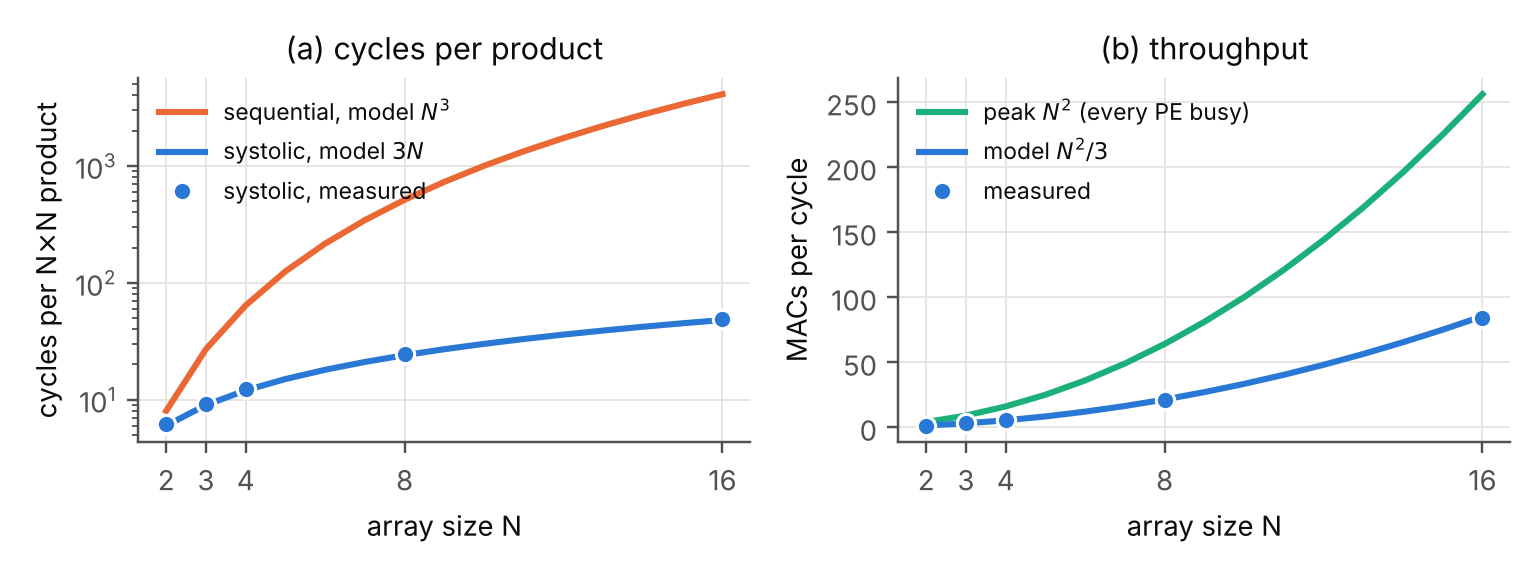
\includegraphics[width=\columnwidth]{fig_scaling.png}
\caption{Array-size sweep: (a) cycles per $N\times N$ product, (b) throughput vs.\ the peak of $N^2$ MACs/cycle.}
\label{fig:scaling}
\end{figure}

The PE utilisation of the OS design is fixed at
$N^3/(N^2\cdot 3N) = 1/3$, independent of $N$
(Fig.~\ref{fig:scaling}b). The wavefront needs $N-1$ cycles to reach the
far corner of the array and $N-1$ cycles to leave it, and the accumulators
must be emptied before the next product, so PEs are idle during both ramps.

% res_comparison.tex  -- written by Shivansh
\subsection{Comparison with the Sequential Baseline}
Table~\ref{tab:compare} and Fig.~\ref{fig:throughput} compare five design
points on a $4\times4$ product, including host data transfer. The compute
kernel alone is 5.4$\times$ faster than the baseline (12 vs.\ 65 cycles).
The Phase~I accelerator, however, is only 1.4$\times$ faster end to end,
because 48 of its 60 cycles move data one element at a time. This is
Amdahl's law in hardware: speeding up the 20\,\% compute part cannot help
the 80\,\% transfer part. Row-wide transfers cut this to 25 cycles.
Overlapping transfers with computation (ping-pong + result buffer) hides
them completely, giving 12.06 cycles per product, i.e.\ the 3N compute
bound. With both pipeline registers the design runs at 116~MHz and
completes a product every 121~ns (1.06~GOPS): 12.4$\times$ faster than the
baseline in wall-clock time.

\begin{table*}[t]
\centering
\caption{Design comparison for one $4\times4\times4$ product (host-visible). $f_{\max}$: post-route, Lattice ECP5-85F (nextpnr). Resources: Yosys \texttt{synth\_xilinx}, Xilinx 7-series.}
\label{tab:compare}
\begin{tabular}{@{}lrrrrrrrr@{}}
\toprule
\textbf{Design} & \textbf{cycles/product} & \textbf{$f_{\max}$ (MHz)} & \textbf{ns/product} & \textbf{GOPS} & \textbf{speed-up} & \textbf{DSP48} & \textbf{LUT} & \textbf{FF}\\
\midrule
Sequential, 1 MAC                 & 113   & 75.7  & 1493 & 0.09 & 1.0$\times$  & 1  & 82   & 40 \\
Phase~I systolic                  & 60    & 55.5  & 1081 & 0.12 & 1.4$\times$  & 16 & 1535 & 1064 \\
Phase~II, serial                  & 25    & 51.3  & 487  & 0.26 & 3.1$\times$  & 16 & 2534 & 1961 \\
Phase~II, overlapped              & 12.06 & 51.3  & 235  & 0.54 & 6.4$\times$  & 16 & 2534 & 1961 \\
Phase~II, overlapped + pipelined  & 14.06 & 116.4 & 121  & 1.06 & 12.4$\times$ & 16 & 3522 & 2284 \\
\bottomrule
\end{tabular}
\end{table*}

\begin{figure}[t]
\centering
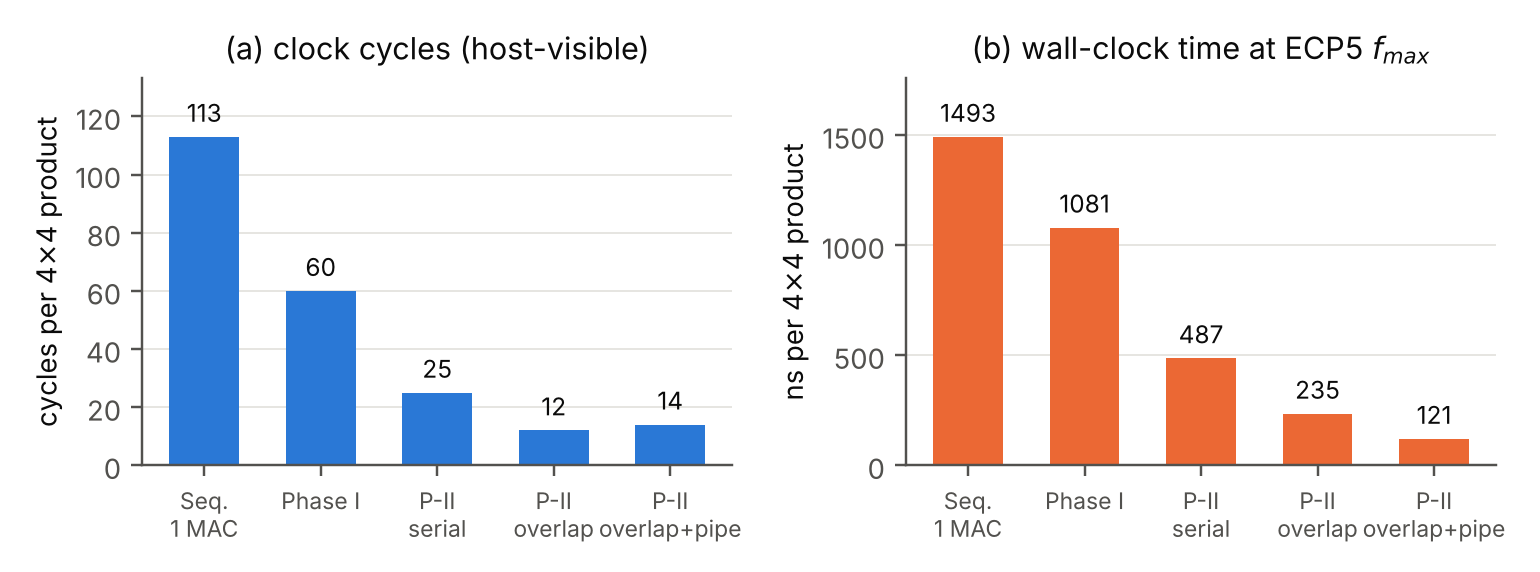
\includegraphics[width=\columnwidth]{fig_throughput.png}
\caption{Cycles and wall-clock time per $4\times4$ product for the five design points.}
\label{fig:throughput}
\end{figure}

The speed-up costs area: 16 DSP blocks instead of 1, and about 3.5\,k LUTs.
Per DSP block the systolic design is slightly less efficient than the
baseline (12.4$\times$ the throughput for 16$\times$ the multipliers),
which matches the 1/3 utilisation discussed above. Its advantage is that
the parallelism scales: at $N=16$ the same structure performs 83.6 MACs per
cycle, while a sequential design is fixed at one.

% res_timing.tex  -- written by Saumya
\subsection{Effect of Overlapping}
Fig.~\ref{fig:wave} shows three consecutive products in overlapped mode.
While the controller is in \textsc{Clear}/\textsc{Feed}/\textsc{Drain}, the
host writes the next $A$ and $B$ (\texttt{wr\_en}) into the inactive bank and
reads the previous result (\texttt{rd\_row} 0--3). A \texttt{done} pulse
occurs every 12 cycles, and the bank pointer alternates.

\begin{figure*}[t]
\centering
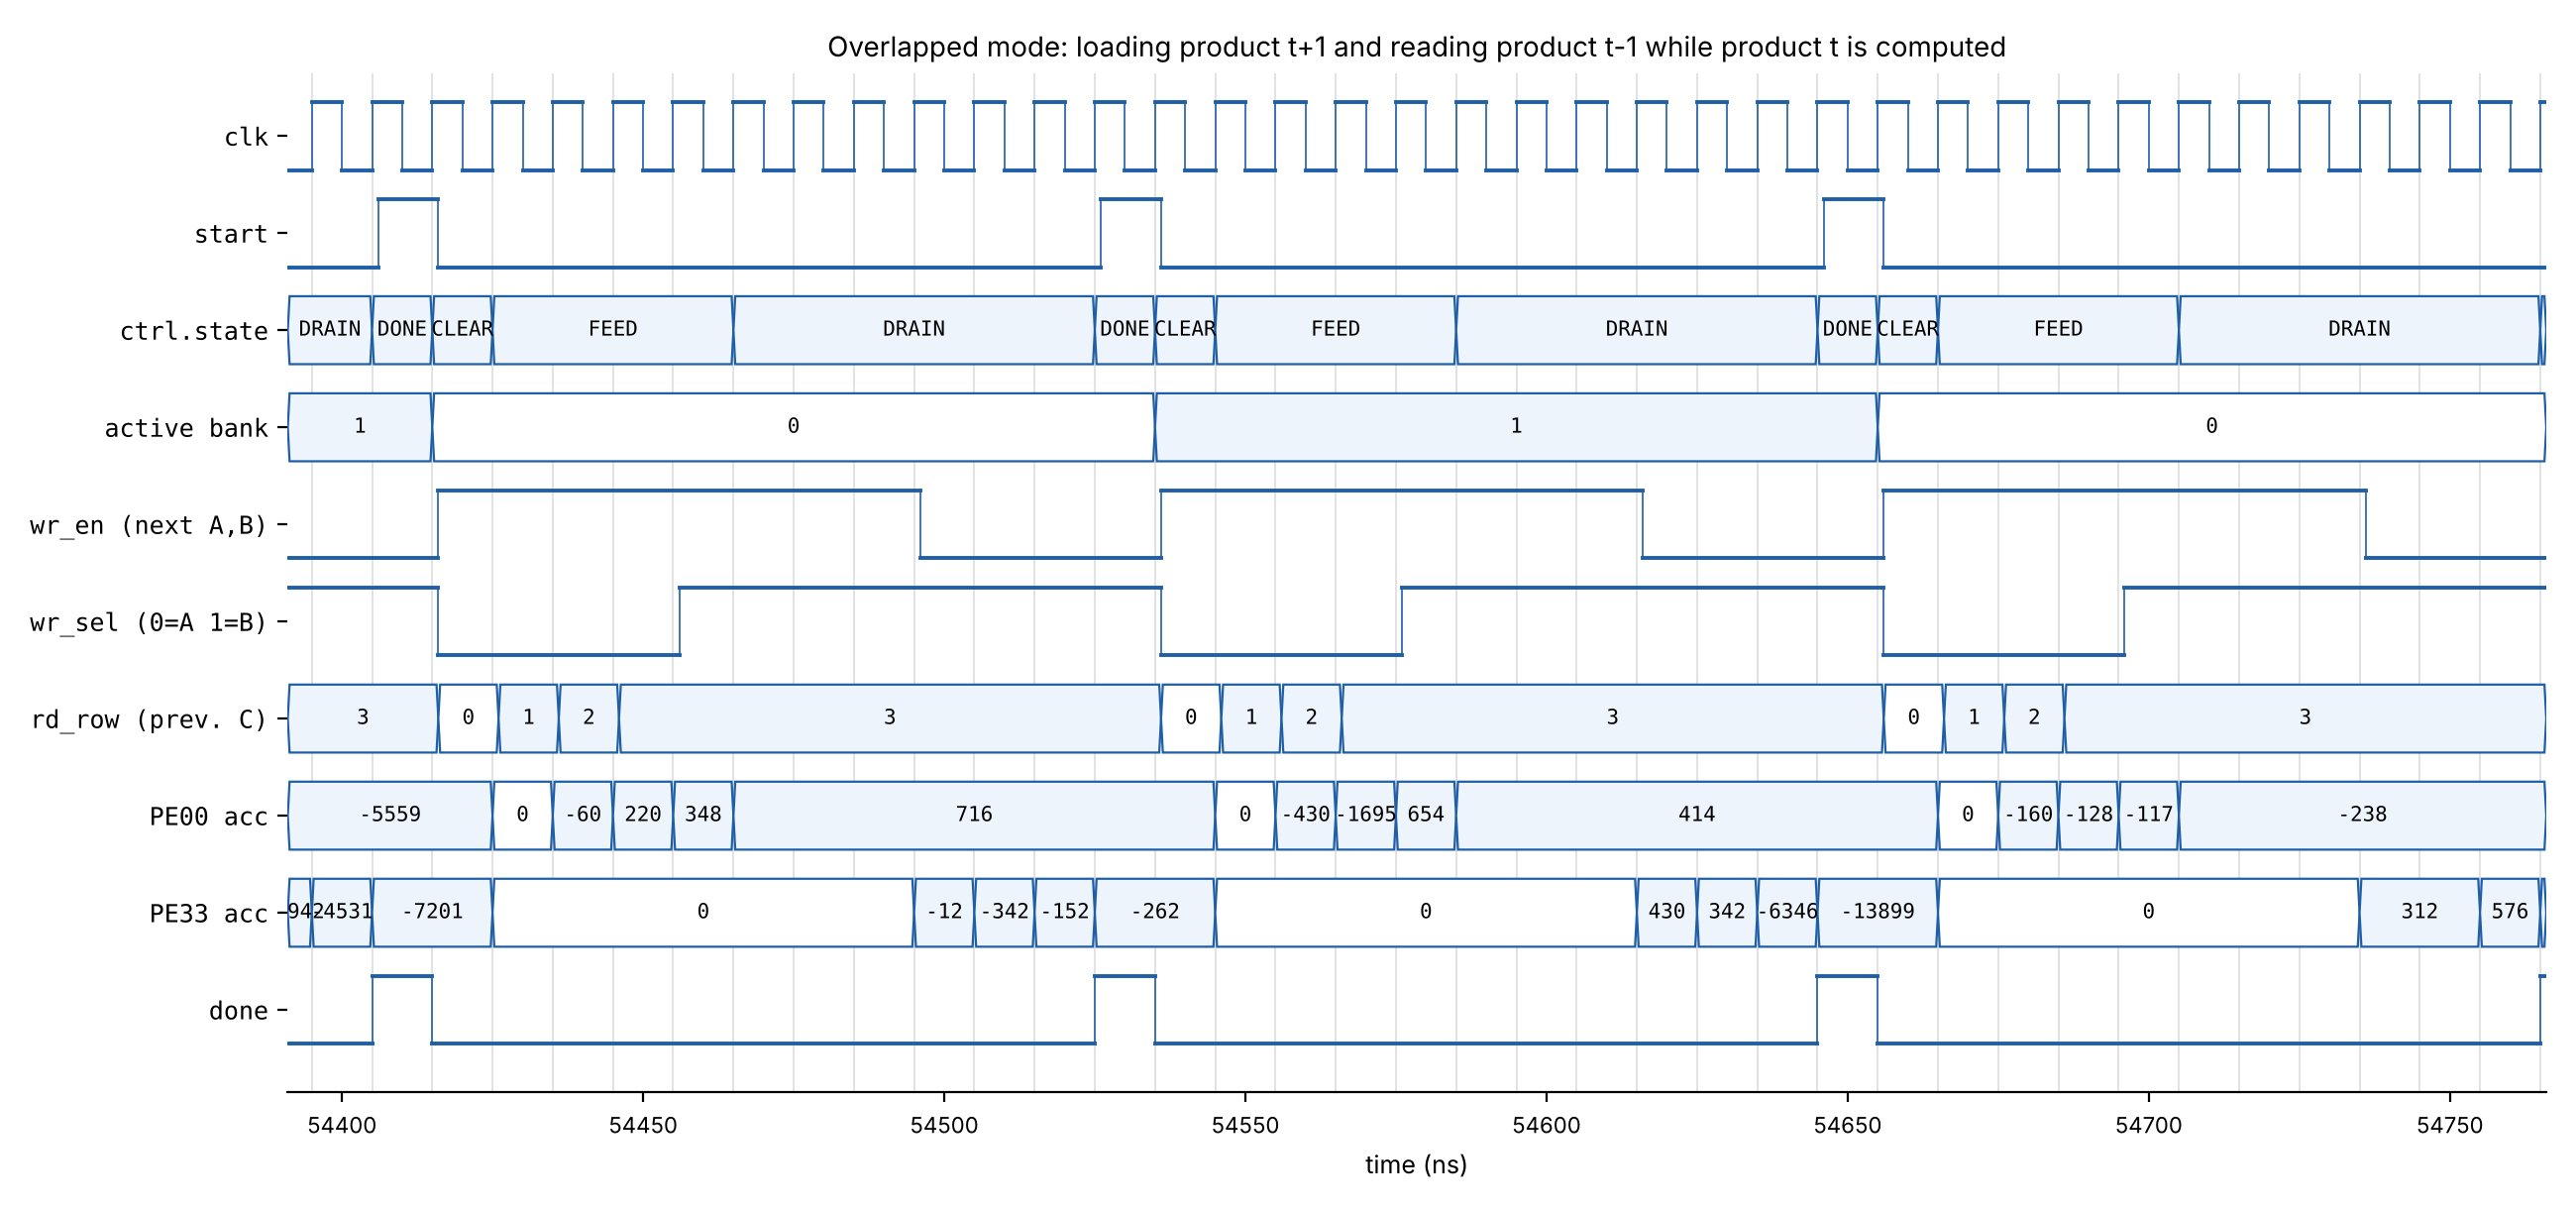
\includegraphics[width=0.95\textwidth]{fig_wave_v2.png}
\caption{Overlapped (streaming) operation of \texttt{systolic\_top\_v2}: host transfers for products $t\pm1$ happen while product $t$ is computed.}
\label{fig:wave}
\end{figure*}

\subsection{Timing Closure and Pipelining}
Without extra registers the design reaches only 51.3~MHz, although an
isolated MAC closes at 193~MHz. The nextpnr critical path runs from the
controller state register, through the feed decode and the buffer read
multiplexer, into the PE$(0,0)$ multiplier and its 32-bit adder. Lane~0 of
the skew logic has no register, so all of these are in series.
Table~\ref{tab:pipe} and Fig.~\ref{fig:pipe} show the effect of the two
optional registers. Each adds one cycle of latency (12$\to$14 cycles per
product) but shortens the critical path. Together they raise $f_{\max}$ by
2.27$\times$ and cut the time per product from 235 to 121~ns. After both
registers, the remaining critical path is one PE forwarding register
feeding the neighbouring DSP multiplier, which is the natural limit of
this structure.

\begin{table}[t]
\centering
\caption{Pipelining study ($N=4$, overlapped, ECP5 post-route)}
\label{tab:pipe}
\setlength{\tabcolsep}{3pt}
\begin{tabular}{@{}lrrrrr@{}}
\toprule
\textbf{registers} & \textbf{latency} & \textbf{cyc/prod} & \textbf{$f_{\max}$} & \textbf{ns/prod} & \textbf{LUT}\\
\midrule
none        & 12 & 12.06 & 51.3  & 235 & 2534 \\
MAC pipe    & 13 & 13.06 & 76.2  & 171 & 3424 \\
buffer reg  & 13 & 13.06 & 70.6  & 185 & 3000 \\
both        & 14 & 14.06 & 116.4 & 121 & 3522 \\
\bottomrule
\end{tabular}
\end{table}

\begin{figure}[t]
\centering
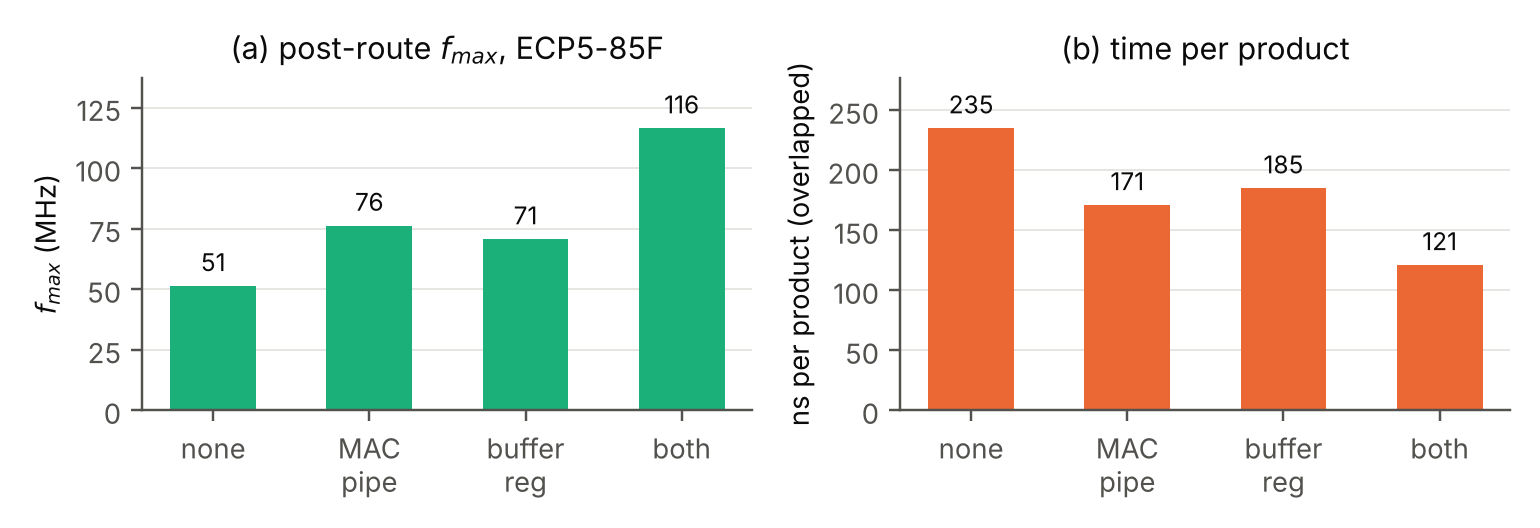
\includegraphics[width=\columnwidth]{fig_pipeline.png}
\caption{(a) Post-route $f_{\max}$ and (b) time per product for each pipeline option.}
\label{fig:pipe}
\end{figure}

\subsection{FPGA Resource Utilisation}
Table~\ref{tab:synth} lists synthesis results. On Xilinx 7-series, Yosys
maps each MAC into one DSP48E1 slice, using the slice's own post-adder as
the accumulator. Without DSPs (\texttt{-nodsp}) a single MAC costs 339
LUTs instead of 32. Phase~II roughly doubles the flip-flops of Phase~I: the
two operand banks add 512~FFs and the result buffer another 512. This is
the price of overlapping. At $N=8$ the design needs 64 DSPs and
10.8\,k LUTs, which still fits a mid-range Artix-7 (e.g.\ XC7A100T with 240
DSPs). The 90 DSPs of an XC7A35T limit that device to $N\le 9$.

\begin{table}[t]
\centering
\caption{Synthesis results (Xilinx 7-series via Yosys; ECP5 post-route via nextpnr)}
\label{tab:synth}
\setlength{\tabcolsep}{2.2pt}
\begin{tabular}{@{}lrrrrr@{}}
\toprule
\textbf{Design} & \textbf{LUT} & \textbf{FF} & \textbf{DSP} & \textbf{ECP5 LUT4} & \textbf{$f_{\max}$}\\
\midrule
MAC (comb.)        & 32    & 32   & 1  & 103   & 193.1 \\
MAC (pipelined)    & 64    & 50   & 1  & 121   & 208.7 \\
MAC, no DSP        & 339   & 32   & 0  & --    & -- \\
Sequential base.   & 82    & 40   & 1  & 203   & 75.7 \\
Phase~I top        & 1535  & 1064 & 16 & 4894  & 55.5 \\
v2, $N=2$          & 842   & 567  & 4  & 2714  & 66.7 \\
v2, $N=4$          & 2534  & 1961 & 16 & 7740  & 51.3 \\
v2, $N=4$, fast    & 3522  & 2284 & 16 & 8034  & 116.4 \\
v2, $N=8$          & 10835 & 7627 & 64 & 29396 & -- \\
WS, $N=4$          & 32    & 859  & 16 & 1269  & 82.9 \\
\bottomrule
\end{tabular}
\end{table}

% res_dataflow.tex  -- written by Harsha
\subsection{Output- vs.\ Weight-Stationary}
For a single $4\times4$ product, OS is faster (12 vs.\ 15 cycles) because
WS must first load its weights. When many rows of $A$ share the same $B$,
as when a neural-network layer is applied to a batch, WS streams them
continuously. It then needs $3N-1+M$ cycles for $M$ rows, against
$\lceil M/N\rceil\cdot 3N$ for OS (Fig.~\ref{fig:osws}a). For $M=16$ WS measures 27 cycles, against about 48 for OS (4 products at
the measured 12.06 cycles each). WS utilisation approaches 100\,\% as $M$ grows,
while OS stays at 33\,\% (Fig.~\ref{fig:osws}b). WS is also cheaper here
(859 FFs, 32 LUTs). Its PE equation $p_{out}=p_{in}+a\cdot w$ maps directly
onto the DSP48 cascade path, and it needs neither operand buffers nor a
result buffer. The costs are 32-bit vertical links instead of 8-bit ones,
the restriction that weights cannot change while rows are in flight, and
the need for an external buffer to supply $A$ rows at full rate. This
explains the TPU's choice of WS for large batched inference. OS remains
attractive when each product has new operands and results must stay local.

\begin{figure}[t]
\centering
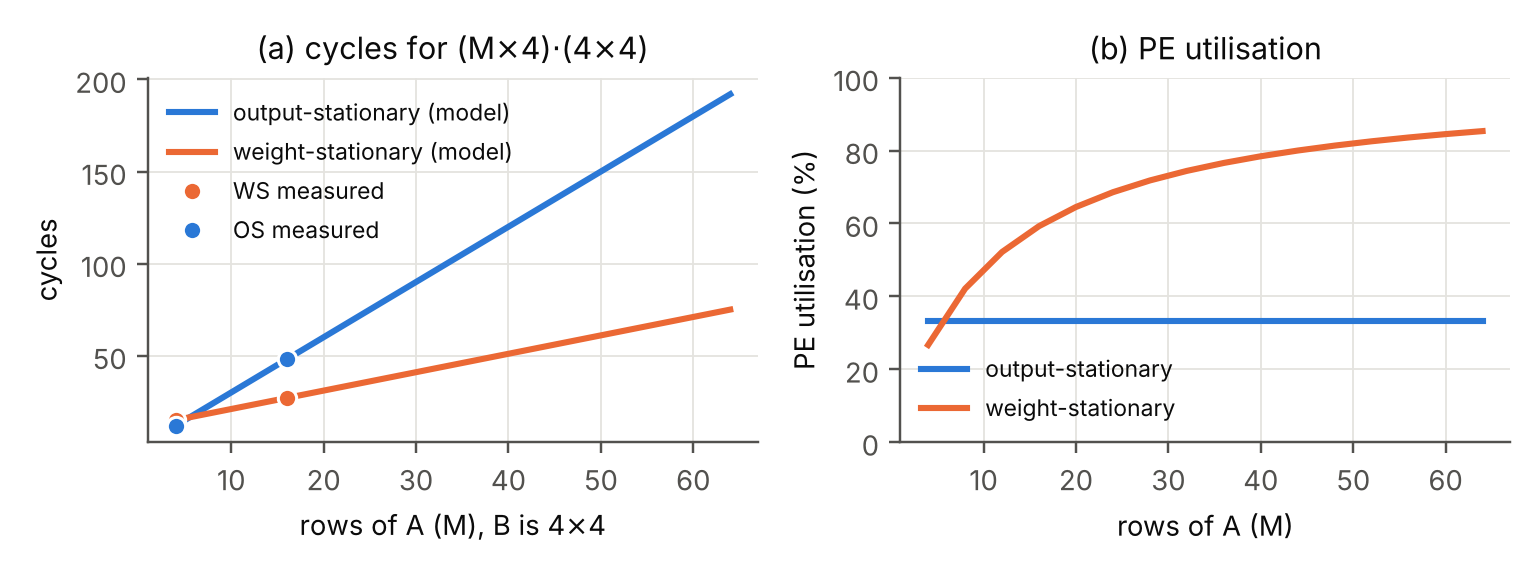
\includegraphics[width=\columnwidth]{fig_os_vs_ws.png}
\caption{OS vs.\ WS for $(M\times4)\cdot(4\times4)$: (a) cycles, (b) PE utilisation.}
\label{fig:osws}
\end{figure}

% res_tiling.tex  -- written by Abhijeet
\subsection{Tiling Larger Matrices}
Accumulate mode lets the $4\times4$ array compute any $S\times S$ GEMM
with $S$ a multiple of 4. The host iterates over output tiles $(I,J)$ and
accumulates $T=S/4$ tile products
$A_{IK}B_{KJ}$ without clearing, while loading the next tiles in parallel.
The $8\times8$ GEMM (8 tile products) takes 105 cycles and the
$12\times12$ (27 tile products) takes 319 cycles. Both match the model of
Section~IV-B exactly. This is 4.9$\times$ and 5.4$\times$ fewer cycles
than the sequential $S^3$, and the array is busy for 80--87\,\% of the
time.

% res_numerics.tex  -- written by Harshvardhan
\subsection{Numerical Accuracy}
Table~\ref{tab:num} compares the fixed-point datapath with float64 over
5000 random products per input distribution. The accumulator itself adds
no error: all error comes from quantising the inputs to Q4.4 (RMSE
0.030 for uniform$[-1,1)$). Requantising to Q4.4 adds only rounding error,
about $0.0625/\sqrt{12}$ per element, giving an RMSE of 0.035
(Fig.~\ref{fig:num}). For larger inputs (uniform$[-2,2)$), 0.3\,\% of the
outputs exceed $\pm8$ and saturate; the \texttt{sat} flags report this to
the host. A Q8.8 output never saturated in these tests.

\begin{table}[t]
\centering
\caption{Accuracy vs.\ float64 (5000 products per distribution)}
\label{tab:num}
\setlength{\tabcolsep}{3pt}
\begin{tabular}{@{}lrrrr@{}}
\toprule
\textbf{Inputs} & \textbf{RMSE Q24.8} & \textbf{RMSE Q4.4} & \textbf{max err Q4.4} & \textbf{sat.\ Q4.4}\\
\midrule
uniform$[-1,1)$ & 0.0295 & 0.0346 & 0.159 & 0.00\,\% \\
uniform$[-2,2)$ & 0.0591 & 0.0617 & 0.255 & 0.30\,\% \\
normal$(0,0.5)$ & 0.0255 & 0.0312 & 0.145 & 0.00\,\% \\
\bottomrule
\end{tabular}
\end{table}

\begin{figure}[t]
\centering
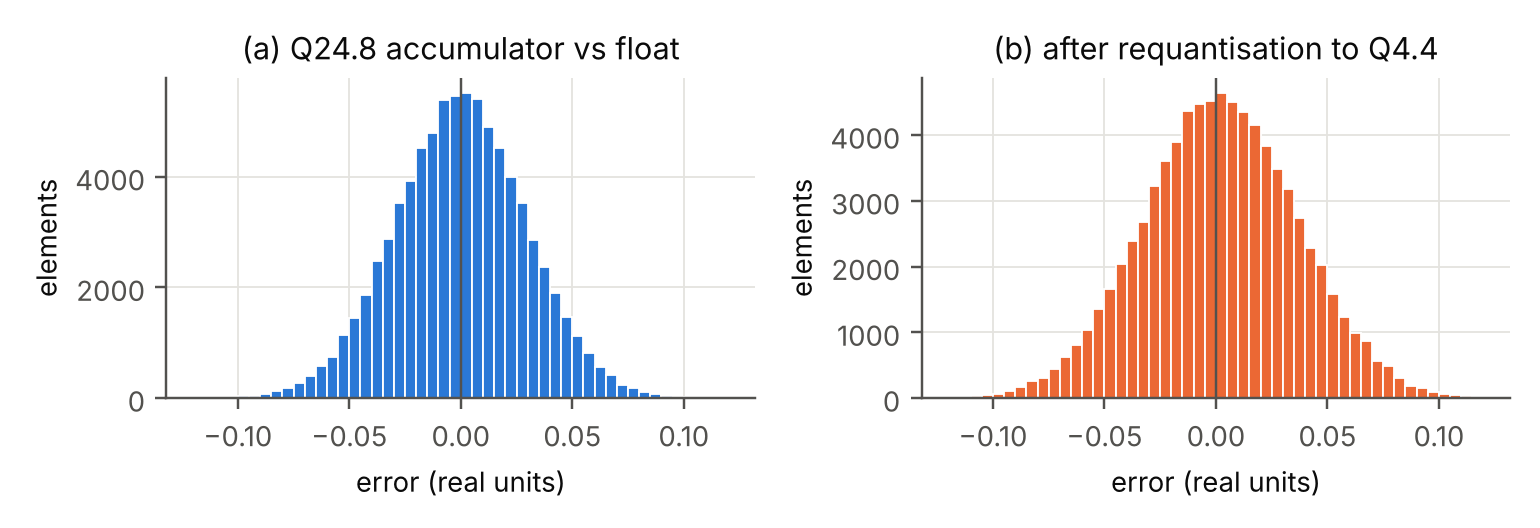
\includegraphics[width=\columnwidth]{fig_numerics.png}
\caption{Error distribution vs.\ float64, uniform$[-1,1)$ inputs.}
\label{fig:num}
\end{figure}

% limitations_conclusion.tex  -- written by Shivansh
\subsection{Limitations}
The FPGA numbers come from an open-source flow: post-route on Lattice ECP5,
and synthesis-level estimates for Xilinx 7-series. Results from the
vendor's own tools for a Xilinx device may differ by tens of percent. The sequential baseline was not pipelined, so its 75.7~MHz
understates what a tuned single-MAC design could reach; the cycle-based
speed-ups (5.4$\times$ compute, 9.4$\times$ end-to-end) do not depend on
this. Finally, the OS design reloads both operands for every product,
which limits utilisation to 1/3, as discussed above.

% -----------------------------------------------------------------------------
\section{Conclusion}
We designed, verified and evaluated a parameterised output-stationary
systolic-array accelerator. The Phase~I prototype showed that the array
computes correctly with a $3N$-cycle latency. Phase~II showed that the
array alone does not determine performance. Data transfer initially
consumed 80\,\% of the time, and only row-wide transfers, double buffering
and a result buffer turned the 5.4$\times$ compute advantage into a real
end-to-end gain. Two pipeline registers then doubled the clock rate. The
final $4\times4$ design completes a product every 14 cycles at 116~MHz
(121~ns): 12.4$\times$ faster than a single-MAC baseline, verified by more
than 85\,000 checks and predicted exactly by a simple analytical model.
The weight-stationary comparison quantified why large accelerators such as
the TPU keep weights in place: utilisation rises from 1/3 towards 1 when
operands are reused across many rows. Natural extensions are a
weight-stationary or hybrid controller with on-chip activation buffers, a
DMA-style memory interface, deeper DSP-internal pipelining and running the
design on an FPGA board.

% contributions.tex  -- written by all members (each edits own row)
\section{Individual Contributions}
Table~\ref{tab:contrib} lists each member's work in both phases. All
members committed their own work from their own GitHub accounts, and each
member can explain the full design.

\begin{table}[h]
\centering
\caption{Individual contributions}
\label{tab:contrib}
\setlength{\tabcolsep}{2.5pt}
\begin{tabular}{@{}p{1.55cm}p{6.35cm}@{}}
\toprule
\textbf{Member} & \textbf{Phase~I / Phase~II} \\
\midrule
Harshvardhan Gupta & I: architecture spec, number format, \texttt{mac\_unit}, MAC testbench, system diagram.
II: \texttt{requant}, pipelined MAC (\texttt{MUL\_PIPE}), \texttt{tb\_requant}, \texttt{tb\_mac\_pipe}, numerical-accuracy study, MAC DSP/LUT synthesis; Abstract, Introduction, numerics results. \\
Harsha Gonela & I: \texttt{pe}, PE testbench, PE figure, literature review.
II: weight-stationary PE/array/top, \texttt{tb\_ws\_top}, OS vs.\ WS analysis and synthesis; Literature Review, dataflow comparison. \\
Abhijeet Dey & I: \texttt{systolic\_array}, \texttt{input\_skew}, array testbench, dataflow figure.
II: accumulate-mode tiling (\texttt{tb\_tiled\_gemm}), array-size sweep (\texttt{tb\_scaling}), analytical performance model (\texttt{perf\_model.py}); latency/throughput and tiling results. \\
Saumya Kumar & I: buffers, controller, Phase~I top, FSM figure.
II: ping-pong buffers, controller v2, perf.\ counters, \texttt{systolic\_top\_v2}, buffer-register timing fix, \texttt{tb\_systolic\_top\_v2}, synthesis/P\&R scripts and timing analysis; architecture and timing sections. \\
Shivansh Upadhyay & I: golden model, system testbench, scripts, report integration.
II: sequential baseline \texttt{seq\_matmul}, 1000-test random regression, golden-model extensions, results tooling (\texttt{plot\_results.py}), comparison results, Conclusion, final report integration. \\
\bottomrule
\end{tabular}
\end{table}


% -----------------------------------------------------------------------------
\begin{thebibliography}{99}

\bibitem{hennessy2019golden}
J.~L. Hennessy and D.~A. Patterson, ``A new golden age for computer
architecture,'' \emph{Commun. ACM}, vol.~62, no.~2, pp.~48--60, Feb. 2019.

\bibitem{sze2017efficient}
V.~Sze, Y.-H. Chen, T.-J. Yang, and J.~S. Emer, ``Efficient processing of deep
neural networks: A tutorial and survey,'' \emph{Proc. IEEE}, vol.~105, no.~12,
pp.~2295--2329, Dec. 2017.

\bibitem{kung1979systolic}
H.~T. Kung and C.~E. Leiserson, ``Systolic arrays (for VLSI),'' in
\emph{Sparse Matrix Proceedings 1978}, SIAM, 1979, pp.~256--282.

\bibitem{kung1982why}
H.~T. Kung, ``Why systolic architectures?'' \emph{Computer}, vol.~15, no.~1,
pp.~37--46, Jan. 1982.

\bibitem{jouppi2017tpu}
N.~P. Jouppi \emph{et al.}, ``In-datacenter performance analysis of a tensor
processing unit,'' in \emph{Proc. 44th Annu. Int. Symp. Comput. Archit. (ISCA)},
2017, pp.~1--12.

\bibitem{jouppi2021tpuv4i}
N.~P. Jouppi \emph{et al.}, ``Ten lessons from three generations shaped
Google's TPUv4i,'' in \emph{Proc. 48th Annu. Int. Symp. Comput. Archit. (ISCA)},
2021, pp.~1--14.

\bibitem{genc2021gemmini}
H.~Genc \emph{et al.}, ``Gemmini: Enabling systematic deep-learning
architecture evaluation via full-stack integration,'' in \emph{Proc. 58th
ACM/IEEE Design Automation Conf. (DAC)}, 2021, pp.~769--774.

\bibitem{samajdar2018scalesim}
A.~Samajdar, Y.~Zhu, P.~Whatmough, M.~Mattina, and T.~Krishna, ``SCALE-Sim:
Systolic CNN accelerator simulator,'' \emph{arXiv:1811.02883}, 2018.

\bibitem{du2015shidiannao}
Z.~Du \emph{et al.}, ``ShiDianNao: Shifting vision processing closer to the
sensor,'' in \emph{Proc. 42nd Annu. Int. Symp. Comput. Archit. (ISCA)}, 2015,
pp.~92--104.

\bibitem{chen2017eyeriss}
Y.-H. Chen, T.~Krishna, J.~S. Emer, and V.~Sze, ``Eyeriss: An energy-efficient
reconfigurable accelerator for deep convolutional neural networks,''
\emph{IEEE J. Solid-State Circuits}, vol.~52, no.~1, pp.~127--138, Jan. 2017.

\bibitem{jacob2018quantization}
B.~Jacob \emph{et al.}, ``Quantization and training of neural networks for
efficient integer-arithmetic-only inference,'' in \emph{Proc. IEEE/CVF Conf.
Comput. Vis. Pattern Recognit. (CVPR)}, 2018, pp.~2704--2713.

\bibitem{patterson_cod}
D.~A. Patterson and J.~L. Hennessy, \emph{Computer Organization and Design:
The Hardware/Software Interface, RISC-V Edition}, 2nd~ed. Cambridge, MA, USA:
Morgan Kaufmann, 2020.

\bibitem{harris_ddca}
D.~M. Harris and S.~L. Harris, \emph{Digital Design and Computer
Architecture}, 2nd~ed. San Francisco, CA, USA: Morgan Kaufmann, 2012.

\bibitem{culler_pca}
D.~E. Culler, J.~P. Singh, and A.~Gupta, \emph{Parallel Computer
Architecture: A Hardware/Software Approach}. San Francisco, CA, USA: Morgan
Kaufmann, 1999.

\bibitem{ieee1364}
\emph{IEEE Standard for Verilog Hardware Description Language}, IEEE Std
1364-2005, 2006.

\bibitem{icarus}
S.~Williams, ``Icarus Verilog,'' [Online]. Available:
\url{https://steveicarus.github.io/iverilog/}

\bibitem{wolf_yosys}
C.~Wolf, ``Yosys Open SYnthesis Suite,'' [Online]. Available:
\url{https://yosyshq.net/yosys/}

\end{thebibliography}

\end{document}
